\begin{answer}
\begin{figure}[H]
  \centering
  \begin{subfigure}[b]{0.49\textwidth}
    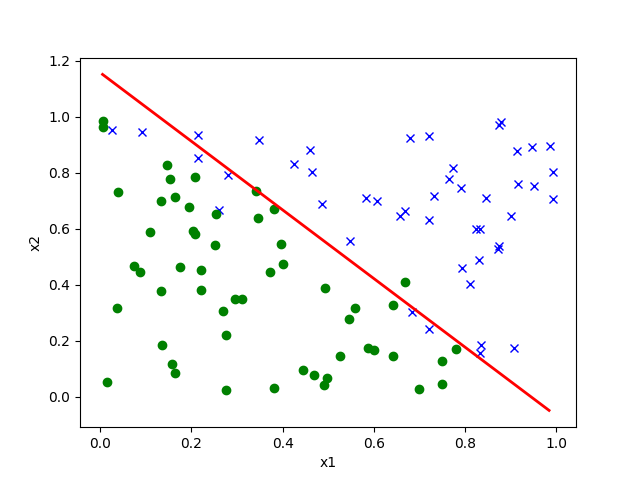
\includegraphics[width=\textwidth]{logreg_stability/logreg_pred_a_reg.png}
    \caption*{Model A with regularization term, $\lambda=0.01$}
  \end{subfigure}
  \begin{subfigure}[b]{0.49\textwidth}
    \includegraphics[width=\textwidth]{logreg_stability/logreg_pred_B_reg.png}
    \caption*{Model B with regularization term, $\lambda=0.01$}
  \end{subfigure}
\end{figure}
\newpage
Without regularization we get final values, $\theta_A = \begin{pmatrix} -20.77957801 &  21.41708931 & 19.81774353\end{pmatrix}$, $\theta_B = \begin{pmatrix} -52.72003622 & 52.90881428 & 52.67579144\end{pmatrix}$\\
With regularization we get final values, $\theta_A = \begin{pmatrix} -2.54018226 & 2.68917584 & 2.19535673 \end{pmatrix}$,\\ $\theta_B = \begin{pmatrix} -2.33368088 & 2.94384675 & 2.3824915 \end{pmatrix}$
\\
We observe that with regularization, the magnitude of the weights is much less, both for A and B.
The decision boundary changes slightly with regularization.
The regularization forces the model to miss-classify some examples in B. This is desirable in cases where the margin of separability is minimal, then the model will not force itself to completely separate the data but should generailize better.
\end{answer}
